\documentclass[11pt]{article}
\usepackage{geometry}                
\geometry{letterpaper}                   

\usepackage{graphicx}
\usepackage{amssymb}
\usepackage{epstopdf}
%\usepackage{natbib}
\usepackage{amssymb, amsmath}
\usepackage{hyperref}
\DeclareGraphicsRule{.tif}{png}{.png}{`convert #1 `dirname #1`/`basename #1 .tif`.png}

%\title{Title}
%\author{Name 1, Name 2}
%\date{date} 

\begin{document}



\thispagestyle{empty}

\begin{center}
\includegraphics[width=5cm]{ETHlogo.eps}

\bigskip


\bigskip


\bigskip


\LARGE{ 	Lecture with Computer Exercises:\\ }
\LARGE{ Modelling and Simulating Social Systems with MATLAB\\}

\bigskip

\bigskip

\small{Project Report}\\

\bigskip

\bigskip

\bigskip

\bigskip


\begin{tabular}{|c|}
\hline
\\
\textbf{\LARGE{Evacuation Bottleneck}}\\
\textbf{\LARGE{A look onto the evacuation of a cruise ship}}\\
\\
\hline
\end{tabular}
\bigskip

\bigskip

\bigskip

\LARGE{Benedek Vartok \& Johannes Weinbuch}



\bigskip

\bigskip

\bigskip

\bigskip

\bigskip

\bigskip

\bigskip

\bigskip

Zurich\\
December 2009\\

\end{center}



\newpage

%%%%%%%%%%%%%%%%%%%%%%%%%%%%%%%%%%%%%%%%%%%%%%%%%

\newpage
\section*{Agreement for free-download}
\bigskip


\bigskip


\large We hereby agree to make our source code for this project freely available for download from the web pages of the SOMS chair. Furthermore, we assure that all source code is written by ourselves and is not violating any copyright restrictions.

\begin{center}

\bigskip


\bigskip


\begin{tabular}{@{}p{3.3cm}@{}p{6cm}@{}@{}p{6cm}@{}}
\begin{minipage}{3cm}

\end{minipage}
&
\begin{minipage}{6cm}
\vspace{2mm} \large Johannes Weinbuch

 \vspace{\baselineskip}

\end{minipage}
&
\begin{minipage}{6cm}

\large Benedek Vartok

\end{minipage}
\end{tabular}


\end{center}
\newpage

%%%%%%%%%%%%%%%%%%%%%%%%%%%%%%%%%%%%%%%



% IMPORTANT
% you MUST include the ETH declaration of originality here; it is available for download on the course website or at http://www.ethz.ch/faculty/exams/plagiarism/index_EN; it can be printed as pdf and should be filled out in handwriting


%%%%%%%%%% Table of content %%%%%%%%%%%%%%%%%

\tableofcontents

\newpage

%%%%%%%%%%%%%%%%%%%%%%%%%%%%%%%%%%%%%%%



\section{Abstract}

This work takes a look onto the evacuation mechanisms of a cruise ship in case of an emergency.
A simple model is implemented, which is used to simulate the dynamics of such a System. 
The main emphasis was on the limited capacity of the exits, since that is the key element for a
rescue boat. 


\section{Individual contributions}

The work on this project was split among us to fit our strengths the best way possible.
Because of his knowledge in image editing and formats, Johannes Weinbuch focused on the 
image manipulation for the input and implemented the loading of the image into MATLAB,
improving the existing solutions from the previous courses. He further took a large part of the writing for the report and executing the simulations, which were written by Benedek Vartok.
He evaluated, which code from previous semesters can and should be reused and implemented the missing parts for our special case. Also, he wrote the output mechanisms for the simulation, so that the data can be used for analysis.


\section{Introduction and Motivations}
In January 2012, the Costa Concordia hit a rock and ran aground\cite{bbcnews}.
This event got great media attention for a long time so we decided to take a closer look
on the evacuation of a cruise ship. The question is, what is the best stratgy to leave the ship?
This question should for sure be answered on one of the emergency drills, but it is always good 
to have some background knowledge.

So, our key questions are: Which is the best strategy for evacuation concerning the choice of the way towards the rescue boats. Should all passengers dirstribute equally over the entries, or is there a better one? Also, which one takes longer: a high panic level on a nearly empty ship or a low panic level on a very full ship. What happens, if a boat suddenly is inoperable? How can the reaction be optimized?

\section{Description of the Model}

The model is a big simplification of real life, otherwise it would be way to complex to simulate.
It assumes, that the ship is intact, that there is calm sea and that the passengers are obliged to leave the ship. 
A possible explanation for this could be a machine defect which leaks explosive gas in a badly ventilated room in the ship. Further, we assume that the rescue boats are like doors, which close after a certain amount of people going through them. 

Since we also assume that the other doors, for example between the rooms or floors, are constantly open and working, we only simulate one deck, the one with the exits to the rescue boats.
The evacuation of multiple floors in a static building has already been researched in \cite{multilevel}. 

After these simplifications, the task left to simulate was the evacuation of a single floor with some elements, that can change.
For this task, we chose a simple agend based modelling solution as described in \cite{helbing}.
A passenger is treated like a particle. It has a mass, and there are physical and social forces, accelerating that mass so that it cannot follow it's desired direction.
The desired direction is implemented as the shortest path to the nearest exit.

The floor is given by a Deck Plan for the Costa Voyager \cite{costa}. Since these deck plans usually are made for advertisment purposes, it is to expect, that they are not absolutely accurate.
So during image processing for simplification of this plan, a few further assumptions were made, mainly about the actual sizes and capacities. 
We won't list them all here, because they are also in the configuration Files. 

The last element of additional complexity was added to get an idea of how the closing of an exit works. 
A switch was added to decide, wether every agent should know instantanously about the closed exit or if the knowledge spreads over time.

\section{Implementation}

\subsection{Input}
Since we had some good projects which covered similar problems as ours, we could get some ideas from them, but at the same time improve them.
Namely, there are \cite{multilevel} and \cite{airplane}. As far as the Input for the simulation is concerned, we see two approaches in these works for getting the map data into the simulation. In \cite{multilevel}, a simple PNG image is used to get a map into the simulation. The Problem here is, that only a certain rgb color value can be read out of the image.
This can lead to problems, if the image is processed with automatic or semiautomatic image manipulation programs, since only a minor difference in color can prevent the generation of the desired data.
In \cite{airplane}, the image format is even more simple. There is only a Bitmap image read into MATLAB. Since the Bitmap Images can use a colormap, Matlab doesn't use 3 channels but a unique Number for each color in a image Matrix to give every Pixel it's color.
This has the same problem as the PNG solution regarding how exactly the colors have to be set, but
the different parts of the image can be separated with less code.

We took the best of both solutions. We used the PNG-Format with indexed Colors.
So we have the most flexibility with very little usage of Disk space.
There is no special ``Wall Color'' or anything like that, just a simple Rule how the Colormap is read:
Color 0 of the map specifies Walls, Color 1 free Space. Then, there can be any Number of Spawn Zones.
Spawn Zones are the areas in the image, where new Agents can be placed. With different Spawn zones, it is possible to account for different situations: A Ball room is different from a Staircase. The number of Spawn Zones is specified in the configuration file. At last, there is any number of exits. Again, each exit can have it's own parameters or can even be handled special in the program's code. 

\begin{figure}[h]
	\centering
	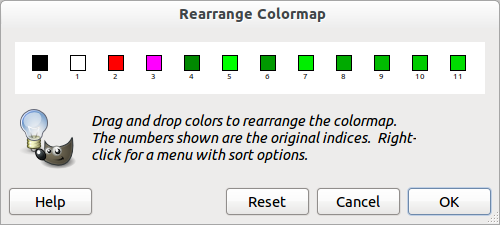
\includegraphics[scale=0.5]{images/gimp.png}
	\caption{Screenshot of the Rearrange Colormap dialog in Gimp 2.6.11}
	\label{gimpscreenshot}
	
\end{figure}
To manipulate the colormap, any slightly sophisticated image manipulation program should suffice. We used the free Software Gimp \cite{gimp}. It has a very comfortable command which allows the user to rearrange the colormap. This is shown in Figure~\ref{gimpscreenshot}.

\subsection{The Simulation Routines} % (fold)
\label{sub:The simulation Routines}

% subsection The simulation Routines (end)

\subsection{Output} % (fold)
\label{sub:Output}

% subsection Output (end)
\section{Simulation Results and Discussion}

\subsection{Passenger distribution} % (fold)
If we plot the exited agents over a time axis for each exit, we can see, that the boats tend to be filled in a sequential way.
This means, a new boat only gets frequented, if the old boad is already full. This effect is very strong and good to see, if we have only few passengers, but also if there are many, a tendency towards this can be observed.
Although there could be numerous reasons for this to happen, in reality a more distributed and parallel filling of the boats is expected. The simulation is based on a model which takes the distance to the nearest exit as the indicator for the desired direction.
In reality, people want to get out of the ship the fastest way possible, especially if there are only limited capacities on the boats.
This suggests, that the nearest exit is not the best strategy to get out fast.
On the specific geometry of the costa Concordia, the corridor from bow to stern ends more on the starboard (right) side. 
The agents follow the shortest path and start to jam up, while on the left, there are no obstacles.
In Reality, at least a few people would recognize that and avoid the jam.
% subsection Passenger distribution (end)

\subsection{Panic Level} % (fold)

% subsection Panic Level (end)
\subsection{Closed exits} % (fold)
\label{sub:Closed exits}
In the simulation, two ways were defined to react to a full boat. First, there was an instantanous update on the whole ship.
This is a model for an announcement over speakers over the whole ship.
The Agents adapt their direction immediately, which can be seen on a video of the simulation.
This behaviour is realistic in a case, when there are not too many people, which are not in panic.

The second way is, that the information is spread in a circle around the exit.
This shall model a simple communication between agents, that takes time.
With this simple rule of updating the directions, the behaviour is much more realistic, even though the rule doesn't account for the number of people nearby. 
This means, the information spreads, even if there is nobody. 
However, an interesting phenomenon during the updates can be observed:
While the people near the exit try to get to the next one, they get pushed back by the others, which don't know of the change yet.

The flaw of this is, that a slow expansion rate leads to more pushing, but if it's too slow, even an agent that escaped can be run against the border of the expansion circle.
This is then seen as the agent stopping, even if there is nothing blocking his path. That happens, because the agent is faster than the expansion rate of the information. From observations in the simulation, we found \(0.5\frac{m}{s}\) to look mostly like we expected it, eventhough sometimes, there are still sometimes agents slowed down by the expansion rate.

The effect of the pushback on the evacuation time is very small, because of numerous bottlenecks before the actual exit.

TODO: PLOT EINFÜGEN

% subsection Closed exits (end)

\section{Summary and Outlook}

\section{References}
\bibliographystyle{plainnat}


\begingroup 
\renewcommand{\section}[2]{}%
\begin{thebibliography}{9}

	\bibitem{bbcnews}
		\url{http://www.bbc.co.uk/news/world-europe-16563562}, 9.12.2012

	\bibitem{multilevel}
	\emph{Modelling Situations of Evacuation
in a Multi-level Building} , 
Hans Hardmeier, Andrin Jenal, Beat Küng, Felix Thaler, Zurich, April 2012

	\bibitem{helbing}
		\emph{Simulating dynamical features of escape panic},
		Dirk Helbing, Ill\'es Farkas, Tam\'as Vicsek, Nature, 28. September 2000

	\bibitem{costa}
		\url{http://www.kreuzfahrtberater.de/deckplan.php?schiff=Costa+Voyager&bf&dpe=2}

	\bibitem{airplane}
		\emph{Pedestrian Dynamics Airplane Evacuation Simulation},
		Philipp Heer, Lukas Bühler, Zurich, May 2011
	\bibitem{gimp}
		\url{http://www.gimp.org/}, 9.12.2012
\end{thebibliography}
\endgroup



\end{document}  



 
